\documentclass{ximera}
\usepgfplotslibrary{fillbetween}
\outcome{Awareness of correspondence between definite integral and area under a curve.}
\outcome{Familiarity with integral notation.}
\outcome{Familiarity with Riemann sum notation.}
\title{Introduction to definite integrals}
\author{Alexander Taam}



\begin{document}
\begin{abstract}
  We motivate, and develop the foundations of, integration.
\end{abstract}
\maketitle

When motivating our study of instantaneous rates of change and differentiation, we considered the problem of calculating (instantaneous) velocity from a given position function. Now we turn our attention to (almost) the opposite problem. \begin{question}If the velocity function of a moving object is given, is it possible determine the position function of the object, or at least calculate the displacement (i.e. change in position) of the object over a given interval?
\end{question}

\begin{fact}
\begin{foldable}
\unfoldable{For simple enough velocity functions, specifically constant functions $v(t)=k$, this is straightforward}. If an object traveling at a constant rate of $k$ meters per second over the time interval $[a,b]$, then $k=\frac{s(d)-s(c)}{d-c}$ for any sub-interval $[c,d]$ of $[a,b]$ where $s(t)$ is the position in meters at time $t$ seconds (of course different choices for units of distance and time may be used as well). In other words\unfoldable{, the instantaneous velocity of the object at any time $t$, $a<t<b$ is equal to the average velocity over any subinterval of $[a,b]$, and so the displacement over a time interval is just the length of the interval times the constant.}
\end{foldable}
\end{fact}

\begin{example}[Displacement from constant instantaneous velocity]
Suppose a car on the highway drives North at $60$ mph for $5$ hours. How far is it to the location of the car after driving for $4$ hours and $15$ minutes, from the location of the car after $1$ hour? \[\answer{195}\]

\begin{feedback} Let $s(t)$ be the distance of the car, in miles, North of its starting point, after driving for $t$ hours. The car travels $60$ miles (in the same direction) each of the three hours: 

from time $t=1$ to $t=2$, 

then from $t=2$ to $t=3$, 

from $t=3$ to $t=4$. 

Finally, in the next quarter hour, from $t=4$ to $t=4.25$, the car travels one quarter of $60$ miles. 

So in total the car travels \[60+60+60+15=3.25\cdot60=s(4.25)-s(1)\] which is exactly the result of solving the equation \[60=\frac{s(4.25)-s(1)}{4.25-1}\] for $s(4.25)-s(1)$.
\end{feedback}
\end{example}

If we graph the constant velocity function $y=v(t)=60$ from the previous example, notice that the displacement over the interval $[1,4.25]$ exactly corresponds to the area of the region between the lines $y=60$, $y=0$, $x=1$ and $x=4.25$.
\[
\graph{y=60\{0< x\},0\leq y\leq 60\{1< x< 4.25\}}
\]

This is not coincidence, in fact, we will see that displacement corresponds to the area under the graph of the velocity function, even for non-constant velocity functions. For this reason we are interested in the following general problem.

\begin{problem}{Net Area Problem}

Given a continuous function $f(x)$ on $[a,b]$, what is the \emph{net area} between the graph $y=f(x)$ and the $x$-axis?

By \emph{net area} we mean the area of the region bounded by $y=f(x)$, the $x$-axis, and the lines $x=a$ and $x=b$, where the area of portions of the region above the $x$-axis count as a positive contribution, and portions below the $x$-axis give a negative contribution.
\end{problem}

\begin{image}
    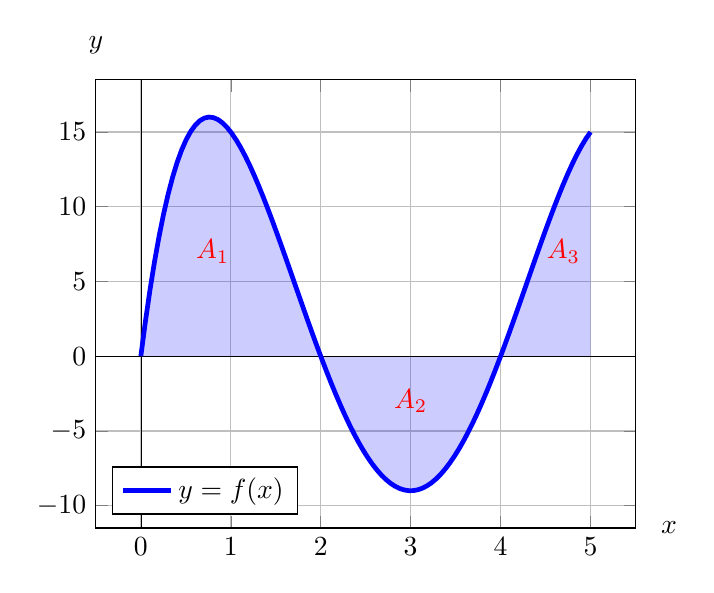
\begin{tikzpicture}
      \begin{axis}[
domain=0:5, 
xlabel=$x$,
ylabel=$y$,
samples=100,grid=major, 
legend pos=south west,
every axis x label/.style={at={(current axis.south east)},right=2mm},
every axis y label/.style={at={(current axis.north west)},above=2mm},
no marks
]
\draw[ultra thin] (axis cs:\pgfkeysvalueof{/pgfplots/xmin},0) -- (axis cs:\pgfkeysvalueof{/pgfplots/xmax},0);
\draw[ultra thin] (axis cs:0,\pgfkeysvalueof{/pgfplots/ymin}) -- (axis cs:0,\pgfkeysvalueof{/pgfplots/ymax});

    \addplot+[name path=A, color=blue, domain=0:5, line width=.6mm] {-1*x*(x-2)*(x-4)*(x-6)}; % actual curve
    \addplot+[draw=none,name path=B] {0};     % “fictional” curve
    \addplot+[thick,
        color=blue,
        fill=blue, 
        fill opacity=0.2] fill between[of=A and B,soft clip={domain=0:5}]; % filling
\node (a) at (axis cs:.8,7)  {\textcolor{red}{$A_1$}};
\node (b) at (axis cs:3,-3)  {\textcolor{red}{$A_2$}};
\node (c) at (axis cs:4.7,7)  {\textcolor{red}{$A_3$}};
\legend{$y=f(x)$}
  \end{axis}
    \end{tikzpicture}
  \end{image}
The net area under $y=f(x)$ from $0$ to $5$ is $A_1-A_2+A_3$

While we generally have a physical intuition for the idea of area that extends beyond squares, triangles, etc. (eg. moving some fixed amount of material into a different shape), we are limited to those shapes for which we know explicit formulas, when attempting calculation. In order to define, and work with areas of more general shapes, calculus is requires.

\end{document}
